% Migrated from the SBCCI/IEEE conference project to the JICS LaTeX template.
% Technical content from the original manuscript was intentionally preserved.
\documentclass[a4paper,10pt,twoside,twocolumn,final]{JICS_LaTexGuidelines}

\RequirePackage{geometry} % Provides margin and dimensions fine-tuning.
\geometry{ % DO NOT MODIFY
    top=1.5 cm,
    left=1.7cm,
    right=1.7cm,
    textheight=25.3cm,
    headsep=0.25cm,
    columnsep=0.6cm,
    footskip=1.2cm
}

\hyphenation{do-cu-ment}

% Packages required by the original SBCCI/IEEE manuscript.
\usepackage{cite}
\usepackage{amsfonts}
\usepackage{amssymb}
\usepackage{algorithmic}
\usepackage{textcomp}
\usepackage{xcolor}
\usepackage{siunitx}
\usepackage{booktabs}
\usepackage{url}

\def\BibTeX{{\rm B\kern-.05em{\sc i\kern-.025em b}\kern-.08em
    T\kern-.1667em\lower.7ex\hbox{E}\kern-.125emX}}

% Original spacing adjustments preserved from the conference manuscript.
\setlength{\abovecaptionskip}{0pt}
\setlength{\belowcaptionskip}{0pt}
\sloppy

\begin{document}

\title{An Auto-Tuning Aging Sensor for FPGA-Based Delay Degradation Monitoring Under Burn-In, Temperature, and Voltage Variations}

\author{L. Nogueira\textsuperscript{1}, D. Alencar\textsuperscript{1}, A. Jaime\textsuperscript{1}, M. Reis\textsuperscript{1}, A. Pamplona\textsuperscript{1}\\
M. Meriaux\textsuperscript{2}, J. A. N. da Silveira\textsuperscript{1}, and F. Vargas\textsuperscript{3}\\
\small
\textsuperscript{1}Universidade Federal do Cear\'a, Fortaleza, Brazil\\
\textsuperscript{2}Polytech Nice Sophia, Biot, France\\
\textsuperscript{3}IHP -- Leibniz Institute for High Performance Microelectronics, Frankfurt (Oder), Germany}

\markboth{Journal of Integrated Circuits and Systems, vol. XX, n. XX, 2026}%
{}%{NOGUEIRA et al.: Auto-Tuning Aging Sensor Under Burn-In Stress}%
\renewcommand*\footnoterule{}%
\footnotetext{Digital Object Identifier 10.29292/jics.vXXiX.X}%
\maketitle

\begin{abstract} The increasing integration of electronic systems in critical applications has made the prediction and mitigation of circuit aging effects a key challenge for ensuring long-term reliability. Traditional solutions such as guard-banding compromise performance, power, area and ultimately cost, highlighting the need for better solutions. This work proposes a self-tuning on-chip aging sensor capable of accurately tracking in-mission critical path time slack erosion, without the need for manual recalibration. The proposed solution enhances a baseline sensor architecture by incorporating a dynamic phase shift mechanism for autonomous slack detection during operation. The sensor was implemented in an FPGA and validated using a comprehensive experimental commercial platform, enabling controlled variation of supply voltage, core temperature, and accelerated aging through burn-in stress. Experimental results showed that the sensor tracks path delay increase under voltage reduction and temperature rise, while continuously monitoring aging effects. Functional failures were observed shortly after the sensor indicated a time slack approaching zero and so, confirming its predictive capability. This approach allows in-mission mode aging monitoring, which is a paramount condition for Silicon Lifecycle Management (SLM) strategies. \end{abstract}





\begin{indexterms}
On-Chip Sensor, Reliability Evaluation, Silicon Lifecycle Management (SLM), FPGA Aging
\end{indexterms}




\section{Introduction}

The continuous demand for higher performance, energy efficiency, and functional integration has made reliability a central design constraint for modern electronic systems. This issue becomes particularly relevant in long-lifetime and safety-critical applications, such as aerospace, automotive, industrial control, medical electronics, and edge-computing platforms, where circuits are expected to operate for several years under non-ideal electrical and environmental conditions. In these scenarios, the correct behavior of a digital system is not only determined by its initial timing closure, but also by the evolution of its timing margin throughout the operational lifetime of the device.

As CMOS technologies have scaled down, reliability margins have become increasingly difficult to preserve. Higher integration density, reduced voltage headroom, increased power density, and stronger process-voltage-temperature (PVT) sensitivity make digital circuits more exposed to both instantaneous operating-condition variations and long-term wear-out mechanisms. Among the most relevant degradation mechanisms, Bias Temperature Instability (BTI), including NBTI and PBTI, Hot Carrier Injection (HCI), electromigration (EM), and Time-Dependent Dielectric Breakdown (TDDB) are commonly associated with transistor- and interconnect-level degradation. These mechanisms may increase threshold voltage, reduce drive current, modify leakage behavior, increase interconnect resistance, and ultimately produce propagation-delay degradation in logic paths \cite{review,Pande2022EMSignalInterconnects,Li2022FPGAAgingPrediction}. In radiation-exposed applications, Total Ionizing Dose (TID) may also induce charge trapping, leakage-current increase, and parametric shifts, which can further reduce timing margins in MOS and FinFET devices \cite{Benfica2016}.

From a system perspective, the most critical consequence of these effects is the progressive erosion of timing slack. A path that is initially timing-safe after manufacturing and static timing analysis may become marginal after prolonged exposure to temperature stress, voltage stress, workload-dependent activity, radiation, or intrinsic aging. Once the path propagation delay approaches the clock-period limit, transient timing errors may occur before the system eventually reaches permanent or recurrent failure. Therefore, the ability to observe slack degradation during operation is an important requirement for resilient systems and for Silicon Lifecycle Management (SLM), whose objective is to combine on-chip telemetry, data analysis, and corrective actions across the lifetime of a device \cite{vargas_and_buff,CNNfabian}.

A conventional mitigation strategy consists of adopting design-time guard-banding, usually by reducing the operating frequency, increasing voltage margins, or imposing conservative timing constraints. Although guard-banding improves robustness, it also introduces direct penalties in performance, power consumption, area, and cost. Furthermore, fixed margins are defined before deployment and cannot accurately reflect the actual degradation rate of each individual device. This limitation is especially important because aging is not uniform across chips, paths, workloads, operating conditions, or spatial regions of the die. Consequently, overly conservative margins may waste performance in healthy devices, while insufficient margins may fail to prevent timing failures in devices exposed to harsher operating conditions.

In this context, on-chip aging and timing-margin sensors have emerged as a more informative alternative to static guard-banding. Rather than assuming a worst-case lifetime margin, these sensors monitor timing degradation directly in the implemented circuit and provide information that can support adaptive voltage and frequency scaling, workload migration, redundancy activation, maintenance scheduling, or predictive failure analysis. Several prior works have proposed aging sensors based on critical-path replicas, delay lines, ring oscillators, shadow flip-flops, phase-shifted sampling, and digital sensor structures \cite{agarwal2007failure,Ernst2004Razor,sensible,valdes,Self_Adjusting_Monitor,Huang2021RealTimeAgingPrediction}. These approaches demonstrate the relevance of runtime observability, but they also expose important practical challenges, such as calibration overhead, dependence on fixed thresholds, limited path representativeness, sensitivity to PVT variations, and the difficulty of validating degradation behavior under controlled physical stress.

FPGA-based platforms are particularly attractive for the experimental study of aging sensors because they provide reconfigurability, accessibility, and a realistic programmable-logic fabric in which timing paths can be implemented, stressed, monitored, and modified. At the same time, FPGAs impose specific implementation constraints that differ from ASIC flows. Placement, routing, clock-domain restrictions, MMCM resources, slice-level clocking constraints, and routing skew can strongly affect the absolute delay observed by a sensor. Therefore, an FPGA-oriented aging sensor must be evaluated not only as a logical monitoring structure, but also as a physically implemented circuit subject to fabric-dependent effects. Prior FPGA aging studies have explored degradation characterization, recycled FPGA detection, accelerated aging through stress configurations, and aging prediction for Xilinx devices \cite{aging_effects_fpga_amouri,short_circuit_aging,WID,Li2022FPGAAgingPrediction}. However, there remains a need for practical FPGA implementations capable of estimating path slack with runtime adjustment and validating the sensor response under voltage, temperature, and accumulated aging stress.

This work addresses this problem by proposing and experimentally validating an auto-tuning on-chip aging sensor for FPGA-based delay-degradation monitoring. The proposed sensor is based on phase-shifted sampling of a monitored path and is enhanced with a Dynamic Phase Shift mechanism implemented through the FPGA clock-management infrastructure. Instead of relying on a statically configured phase offset, the sensor automatically shifts the sampling clock until an alarm is triggered, allowing the system to estimate the available slack of the monitored path. In this way, the sensor is not limited to detecting that a fixed degradation threshold has been reached; it can also provide a digital measurement associated with the current timing margin. This feature is important for mission-mode monitoring because the sensor can be recalibrated during operation and can track slack evolution as a function of stress, operating conditions, or lifetime.

The experimental validation is performed on a Xilinx Artix-7 FPGA implemented on a Nexys 4 DDR development board. The monitored Circuit Under Test (CUT) is based on an arithmetic datapath designed to generate controlled and repeatable switching activity, while a reference computation is used to identify functional timing errors. The proposed sensor is evaluated under controlled supply-voltage variation, core-temperature variation, and accelerated aging through burn-in stress. The experimental setup combines an externally supplied FPGA core voltage, thermal stress, on-chip XADC measurements, host-side data acquisition, and sensor phase-shift monitoring. This methodology allows the sensor response to be correlated with voltage, temperature, and accumulated stress conditions.

The obtained results show that the proposed sensor tracks timing-margin variations coherently with the applied stress conditions. Voltage reduction and temperature increase lead to lower measured slack, indicating slower path behavior, while higher voltage and lower temperature increase the available timing margin. After accelerated burn-in stress, the monitored path exhibits systematic slack reduction across the evaluated operating corners. Moreover, functional timing failures are observed only after the sensor indicates a slack value close to zero, supporting the use of the proposed structure as an early indicator of timing-margin exhaustion. These results suggest that the sensor can provide useful runtime information for SLM-oriented strategies in FPGA-based systems.

The remainder of this paper is organized as follows. Section II presents the proposed sensor architecture, the dynamic phase-shift auto-tuning mechanism, FPGA implementation considerations, the CUT, and the experimental setup. Section III presents and discusses the voltage, temperature, burn-in, and functional failure characterization results. Finally, Section IV concludes the paper and outlines future research directions.

\section{Related Works}

Aging detection and monitoring have been extensively studied in the context of digital integrated circuits. A recent survey by Lanzieri \textit{et al.} \cite{review} organizes aging-monitoring techniques for embedded systems and reinforces that aging is a cross-layer problem involving physical degradation mechanisms, circuit-level symptoms, architectural exposure, and system-level mitigation. From the circuit perspective, most aging mechanisms become critical when they modify the timing response of the system. BTI and HCI mainly affect transistor parameters and drive strength, while EM and interconnect degradation can increase resistance and modify delay distribution along signal paths. In advanced devices, these effects are aggravated by reduced timing margins and stronger dependence on PVT conditions \cite{introduction_amouri,Pande2022EMSignalInterconnects,Li2022FPGAAgingPrediction}.

A classical line of work addresses timing-error detection and failure prediction. Agarwal \textit{et al.} \cite{agarwal2007failure} showed that circuit failure prediction can be used to anticipate transistor-aging-induced timing failures before functional malfunction. Razor \cite{Ernst2004Razor} demonstrated that timing errors can be detected at circuit level through a main flip-flop and a delayed shadow element, enabling dynamic voltage scaling at the cost of recovery mechanisms and architectural support. These works established an important principle: timing degradation should be observed close to the functional datapath, because the final reliability concern is not the isolated physical mechanism, but whether the path can still meet its timing constraint.

Several subsequent works proposed on-chip sensors for aging and delay monitoring. Valdes-Pe\~na \textit{et al.} \cite{valdes} presented configurable online aging sensors for nanometer-scale FPGAs based on phase-shifted sampling. SENSIBle \cite{sensible} proposed a scalable sensor design for path-based age monitoring in FPGAs, focusing on the selection and monitoring of representative paths. Sadeghi-Kohan \textit{et al.} \cite{Self_Adjusting_Monitor} introduced a self-adjusting monitor for measuring aging rate and advancement, reinforcing the need to extract more information than a single binary indication of degradation. More recently, Vargas \textit{et al.} \cite{Base_Sensor} proposed an on-chip sensor to monitor aging evolution in FinFET-based memories, and Vargas and Balakrishnan \cite{vargas_and_buff} discussed an on-chip aging sensor core in the context of SLM. These works are directly related to the sensor principle adopted in this paper, but most approaches still rely on predefined thresholds, static phase configuration, or validation scenarios that do not fully combine runtime slack estimation with empirical burn-in, temperature, and voltage stress on a commercial FPGA platform.

Another relevant direction is the use of digital sensors and predictive methods for degradation analysis. Huang \textit{et al.} \cite{Huang2021RealTimeAgingPrediction} proposed real-time IC aging prediction using on-chip sensors to record historical operating-condition parameters and estimate aging-related degradation. Chen \textit{et al.} \cite{chen2022solar_prediction} explored the use of monitored hardware information and supervised machine learning for reliability prediction in radiation-sensitive systems. Although this second work is focused on solar particle events and single-event upsets, it reinforces a broader trend in reliable-system design: raw sensing is only the first layer of a monitoring flow, and sensor outputs should be suitable for higher-level prediction, adaptation, or maintenance decisions. The present work is aligned with this trend because the proposed sensor provides a quantitative slack-related indicator, rather than only a fixed alarm, which can later be used as input to predictive models.

FPGA aging characterization has also received attention because programmable devices are widely used in prototyping, space systems, industrial platforms, and long-lifetime reconfigurable computing. Amouri \textit{et al.} \cite{aging_effects_fpga_amouri} experimentally analyzed aging effects in FPGAs, while Gaskin \textit{et al.} \cite{short_circuit_aging} proposed accelerated FPGA aging through novel configuration techniques that stress the programmable fabric. Ahmed \textit{et al.} \cite{WID} explored recycled FPGA detection using exhaustive fingerprinting assisted by within-die process variation modeling. Li \textit{et al.} \cite{Li2022FPGAAgingPrediction} investigated aging mechanism analysis and prediction for Xilinx 7-series FPGAs fabricated in a 28-nm process. These works demonstrate that FPGA aging can be induced, measured, and modeled, but they are primarily focused on aging characterization, detection of recycled devices, or device-level degradation analysis. In contrast, this work focuses on a path-level timing-margin sensor that can be integrated with the monitored logic and dynamically calibrated during operation.

Burn-in and accelerated aging procedures are commonly used to expose latent defects and accelerate wear-out mechanisms under elevated temperature and voltage stress. Standards such as MIL-STD-883 Method 1015, MIL-STD-883 Method 1005, and JEDEC JESD22-A108 define temperature, bias, and operating-life procedures that are frequently used as references for accelerated reliability evaluation \cite{milstd883_1015,milstd1005SSL,jedecA108D}. In FPGA-oriented studies, accelerated aging may be performed by increasing temperature, increasing supply voltage, increasing activity, or combining these stressors. However, there is still a practical gap between accelerated-aging procedures and runtime-capable sensor validation. Many works either characterize degradation after stress or evaluate sensor structures without exposing the device to a complete physical stress methodology. The present work contributes to this point by validating the sensor under controlled voltage and temperature sweeps and after accumulated burn-in stress, allowing the measured slack degradation to be compared under equivalent operating corners.

Finally, recent SLM-oriented works emphasize that future dependable systems require continuous telemetry and hardware/software interfaces capable of transforming sensor information into decisions. Vargas and Balakrishnan \cite{vargas_and_buff} discuss aging-sensor structures as support elements for SLM, while Syed \textit{et al.} \cite{CNNfabian} explore resilience in reconfigurable CNN accelerators using a multi-purpose on-chip sensor. These works indicate that aging sensors should not be treated as isolated test structures, but as elements of a broader monitoring infrastructure. Considering this context, the main gap addressed in this paper is the lack of a practical FPGA-based aging-monitoring solution that simultaneously provides runtime slack estimation, auto-tuning through dynamic phase shifting, and empirical validation under voltage, temperature, and burn-in stress.

\subsection{Key Contributions of This Work}

Considering the related work discussed above, the key contributions of this work are summarized as follows:


\noindent\textbf{C1 -- Auto-tuning slack monitoring:} The proposed FPGA-oriented aging sensor uses the dynamic phase-shift capability of the clock-management infrastructure to automatically identify the sampling threshold associated with the available path slack.

\noindent\textbf{C2 -- Mission-mode self-calibration:} Unlike fixed-threshold sensors, the proposed approach can recalibrate the phase-shifted sampling clock during operation, enabling the monitored slack to be tracked over time and supporting SLM-oriented strategies.

\noindent\textbf{C3 -- FPGA implementation analysis:} The work discusses practical implementation constraints in FPGA fabrics, including placement proximity, routing skew, slice-level clock-domain restrictions, and the interpretation of relative slack variations.

\noindent\textbf{C4 -- Empirical validation under stress conditions:} The sensor is validated on a commercial Artix-7 FPGA platform under voltage variation, temperature variation, and accelerated burn-in stress, allowing slack evolution to be correlated with controlled operating corners.

\noindent\textbf{C5 -- Correlation with functional timing failure:} The experimental results show that functional timing errors occur only after the sensor indicates slack close to zero, reinforcing its use as an early warning mechanism for timing-margin exhaustion.





\section{Methodology}\label{sec:methodology}

\subsection{Proposed Aging Sensor: Architecture and Operating Principle}
\label{sec:sensor_architecture}

The sensor architecture employed in this work is based on the structure proposed in \cite{Base_Sensor}, and is illustrated in Figure~\ref{fig:sensor}. The circuit is designed to monitor the timing margin of a selected path by comparing samples taken with the system clock and with an intentionally phase-shifted clock.

The circuit comprises two sampling flip-flops: FF\_sys\_clock, which receives the system's main clock signal (\textit{sys\_clk}), and FF\_psclk, which receives a phase-shifted clock (\textit{psclk}), advanced with respect to \textit{sys\_clk}. Both flip-flops sample the signal propagated through the monitored path. The outputs of these flip-flops are compared using an XOR gate. If the sampled values are equal, the XOR output remains at a LOW logic level; otherwise, it transitions to a HIGH level.

\begin{figure}[htbp!]
    \centering
    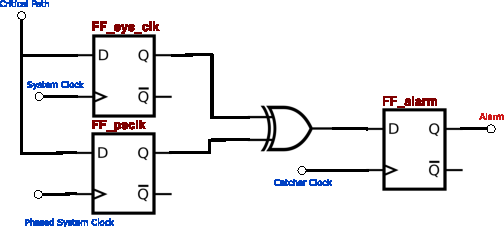
\includegraphics[width=0.8\columnwidth]{Figures/sensor.pdf}
    \caption{\small Logical structure of the aging sensor, composed of flip-flops, XOR gate, and phase-shifted clocks.}
    \label{fig:sensor}
\end{figure}

The XOR output is then sampled by a third flip-flop, FF\_alarm, which is triggered by a delayed clock referred to as the \textit{catcher clock}. This clock is lagged with respect to the main clock to provide sufficient time for the propagation and stabilization of the comparison logic. When the XOR output indicates a mismatch at the rising edge of the \textit{catcher\_clock}, the alarm is triggered and remains active until a reset signal is asserted.

The functional goal of the sensor is to estimate the slack of the monitored path, defined as the difference between the clock period and the path propagation delay. To determine this slack, the sensor undergoes a calibration process. Initially, \textit{psclk} is aligned with \textit{sys\_clk} and then progressively shifted to the left, i.e., advanced with respect to the system clock. This shifting continues until the alarm is triggered. The instant at which the alarm is activated indicates that \textit{psclk} has reached the boundary of the available timing margin. Therefore, the applied phase shift at the alarm threshold corresponds to the estimated slack of the monitored path.

Figures~\ref{fig:path} and~\ref{fig:aged_path} illustrate the timing behavior of the signals involved in the sensor operation. Figure~\ref{fig:path} presents a scenario in which the sensor is calibrated and the monitored path has not yet undergone delay degradation. In this case, the path transition still occurs within the available slack, and the alarm is not triggered. Conversely, Figure~\ref{fig:aged_path} depicts a situation in which the propagation delay of the monitored path has increased. Under the same calibration condition, the delayed transition is captured differently by the two sampling flip-flops, producing a mismatch and activating the alarm.

\begin{figure}[htbp!]
    \centering
    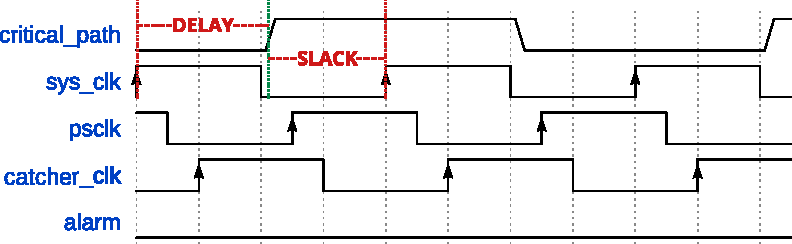
\includegraphics[width=0.8\columnwidth]{Figures/path.pdf}
    \caption{\small Timing diagram of the sensor operation when the monitored path has not undergone delay degradation, showing the combinational delay and the available slack. Alarm not triggered.}
    \label{fig:path}
\end{figure}

\begin{figure}[htbp!]
    \centering
    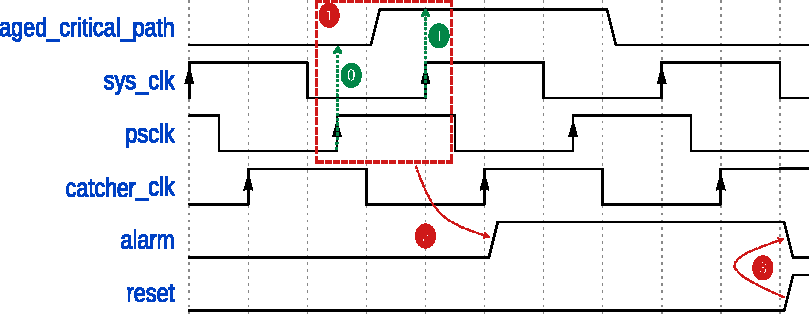
\includegraphics[width=0.8\columnwidth]{Figures/aged_path.pdf}
    \caption{\small Timing diagram of the sensor operation under delay degradation: (1) the input flip-flops capture distinct values, resulting in (2) the activation of the alarm, which remains active until (3) the reset signal is asserted.}
    \label{fig:aged_path}
\end{figure}


\subsection{Proposed Aging Sensor: Dynamic Phase Shift and Auto-Tuning Mechanism}
\label{sec:sensor_autotuning}

In the conventional approach, sensor calibration is performed statically by defining the phase of \textit{psclk} during the FPGA configuration stage. In this scenario, once the alarm is triggered, it is only possible to conclude that the available \textit{slack} has decreased, without the ability to recalibrate the sensor unless the FPGA is reprogrammed. Based on this limitation, this work proposes an adaptation and enhancement of the original sensor architecture.

By employing the dynamic phase shift mechanism available in the MMCMs (Mixed-Mode Clock Managers) of Xilinx 7 Series FPGAs and later families, it becomes possible to perform precise runtime adjustments to the phase of a clock relative to a reference. The configuration procedure and the calculation of phase resolution per increment are detailed in \cite{xilinxUG472}. In this work, each increment was configured to correspond to a phase shift of \SI{19.85}{\pico\second}. The greater the number of increments applied, the larger the resulting phase shift.

Applying this mechanism to \textit{psclk}, using \textit{sys\_clk} as a reference, enables the use of internal control signals to automatically estimate the \textit{slack}. Moreover, it allows the sensor to be recalibrated at runtime whenever a variation in the monitored path delay is detected. Figure~\ref{fig:dynamic_shift} illustrates this progressive phase-shifting principle: at each calibration step, the sampling clock (\textit{psclk}) is advanced with respect to the previous step by one additional phase-resolution increment $X$, so that the accumulated shift after $n$ steps corresponds to $n \cdot X$.

\begin{figure}[htbp!]
    \centering
    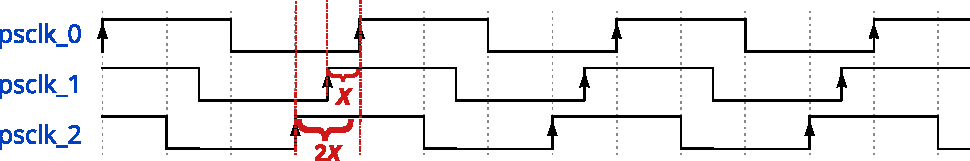
\includegraphics[width=0.8\columnwidth]{Figures/dynamic shift.pdf}
    \caption{\small Progressive phase-shift steps applied to the sampling clock during auto-tuning. Each successive waveform (\textit{psclk\_0}, \textit{psclk\_1}, \textit{psclk\_2}, \ldots) is advanced by one additional increment $X$ with respect to the previous one, so the accumulated shift grows as $X$, $2X$, and so on until the alarm is triggered.}
    \label{fig:dynamic_shift}
\end{figure}

The control flow of the sensor's self-calibration mechanism is illustrated in Figure~\ref{fig:sensor_state_machine}. Initially, \textit{psclk} is aligned with \textit{sys\_clk}. The controller continuously monitors the sensor's alarm signal. While the alarm remains inactive, the controller issues commands to the MMCM to increment the phase of \textit{psclk}, gradually shifting it to the left. This process is repeated until the alarm is triggered. At that point, the controller records the number of increments applied. By multiplying this number by the phase resolution per increment, the slack value is calculated in picoseconds.

Once the calibration process is complete, the sensor is considered calibrated, and the controller remains in an idle state until a \textit{reset} signal is received. This signal reinitializes the state machine, realigns the clocks, and restarts the calibration procedure. The frequency of the \textit{reset} signal should be defined according to the monitoring requirements of the target system.

\begin{figure}[htbp!]
    \centering
    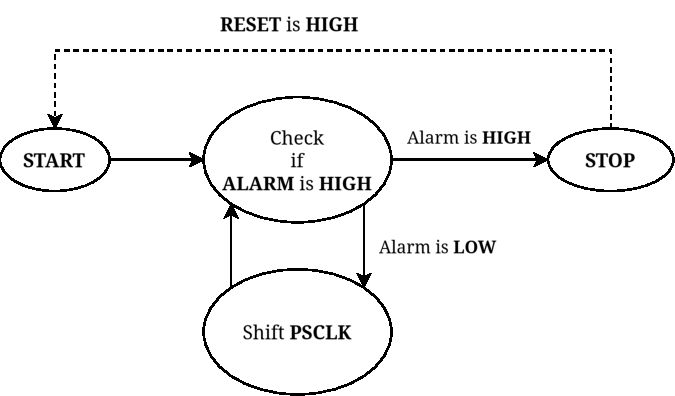
\includegraphics[width=0.8\columnwidth]{Figures/FSM.pdf}
    \caption{\small State machine diagram of the sensor's self-calibration controller.}
    \label{fig:sensor_state_machine}
    
\end{figure}


\subsection{Proposed Aging Sensor: Delay-Centric Monitoring and Slack Interpretation}
\label{sec:sensor_delay_centric_monitoring}

The proposed sensor does not attempt to identify the physical origin of a timing-margin variation. Instead, it directly observes the final electrical consequence of different stress sources: a change in the propagation delay of the monitored path and, consequently, a reduction of its available slack. This is a useful property because several independent phenomena can converge to the same circuit-level manifestation. Variations in operating temperature and supply voltage modify transistor drive strength and interconnect behavior, while localized hotspots introduce spatially non-uniform delay shifts across the die. Similarly, operation under aggressive conditions, such as overclocking or over-voltage stress, can either reduce the available timing budget or accelerate device wear-out. Time-dependent degradation mechanisms, including NBTI/PBTI, HCI, and electromigration, also manifest at circuit level as threshold-voltage shifts, drive-current degradation, interconnect-resistance increase, or timing-error-rate degradation \cite{Lanzieri2024AgeingSurvey,Pande2022EMSignalInterconnects,Huang2021RealTimeAgingPrediction}.

For this reason, the sensor remains effective under the highlighted scenarios because its detection criterion is delay-centric rather than mechanism-centric. A temperature rise, a hotspot, a voltage-induced operating shift, or long-term wear-out will be detected whenever its net effect moves the monitored path transition into the configured guard band. In other words, the sensor measures the timing symptom that matters for correct operation: the proximity of the path delay to the clock-period limit. This makes the approach complementary to environmental telemetry, such as on-chip temperature and voltage monitors. While those monitors help correlate or classify the root cause of the observed degradation, the proposed sensor provides direct evidence that the actual implemented path is losing timing margin under the current operating and aging conditions \cite{AMD_DS931_ArtixUltraScalePlus_2026,Li2022FPGAAgingPrediction,Lanzieri2024AgeingSurvey}.

The interpretation of the sensor response must therefore be performed by comparing slack measurements obtained under equivalent operating conditions. Since temperature, supply voltage, workload, and localized thermal gradients can also affect path delay, aging-related degradation is inferred from timing-margin shifts observed when these variables are controlled or properly accounted for. In this context, the sensor provides a direct measurement of the delay variation experienced by the monitored path, while the experimental protocol defines the conditions under which this variation can be attributed to long-term wear-out rather than to instantaneous environmental fluctuations.

Accordingly, in this work, slack degradation is evaluated by comparing sensor responses under controlled burn-in, temperature, and voltage conditions. This allows the observed timing shift to be associated with aging-induced degradation, independently of the specific underlying physical mechanism involved, such as NBTI/PBTI, HCI, or electromigration. Thus, the sensor is used as a timing-margin monitor, and the attribution of the measured slack reduction to aging is supported by consistent operating-condition comparisons throughout the experimental analysis.


\subsection{Proposed Aging Sensor: Activity and Aging Exposure Management}
\label{sec:sensor_activity_aging}

It is also important to consider the aging exposure of the monitoring circuitry itself. Aging-induced slack degradation is typically a slow process, evolving over long operating periods rather than over short execution windows. Therefore, the sensor should be operated in a way that avoids turning the monitoring circuit into an aged reference. In an ASIC implementation, this can be addressed by power-gating the distributed sensor blocks during idle intervals, disconnecting them from the supply rails and enabling them only during periodic monitoring or calibration phases. This strategy virtually eliminates both switching activity and static bias stress while the sensor is inactive, and should therefore be employed whenever fine-grained power-gating is available.

In FPGA-based implementations, however, arbitrary fine-grained power-gating of user logic is generally not available in the same way as in ASIC flows. Although some FPGA families may include architecture-specific power-management features for selected hard blocks or unused resources, the programmable logic implementing the proposed sensor normally remains connected to the device power rails. For this reason, the recommended FPGA-oriented mitigation is to gate the sensor clock and control activity whenever monitoring is not required. In UltraScale/UltraScale+ devices, for example, clock-enable resources and clock-buffer primitives such as BUFGCE can be used to suppress unnecessary clock toggling in a controlled manner \cite{AMD_UG572_UltraScaleClocking_2025}. This does not remove leakage or all bias-related stress, as power-gating would, but it substantially reduces the sensor activity factor and the corresponding switching-related stress.

Moreover, the sensor is inserted in parallel with the monitored circuit and is not part of the functional datapath. Consequently, its activity profile is defined by the monitoring policy rather than by the workload of the protected logic. If the sensor is activated only during short observation windows, its effective duty cycle can be made much smaller than that of the monitored path. Under this usage model, the residual degradation of the sensor becomes negligible with respect to the degradation being tracked in the functional logic, preserving the sensor as a stable timing reference for long-term slack monitoring \cite{Jahanirad2023DPGFPGA,Li2022FPGAAgingPrediction}.


\subsection{Proposed Aging Sensor: FPGA Implementation Considerations}
\label{sec:fpga_considerations}

It is important to highlight the design considerations and necessary adaptations for the physical implementation of the sensor on FPGAs. First, the sensor should be placed as close as possible to the output of the monitored path. The greater the distance, the higher the interconnection delay will be. Ideally, the total delay observed by the sensor should be dominated by the logical delay of the monitored path itself. Increased routing delay reduces the accuracy of the \textit{slack} estimation and may introduce implementation-dependent offsets.

Additionally, the sensor logic requires one LUT2 to implement the XOR gate and three flip-flops, each operating under a distinct clock domain. Since each FPGA \textit{slice} can only be driven by a single clock, the flip-flops must be placed in separate \textit{slices}. Therefore, at least three distinct \textit{slices} are required to implement the sensor.

Finally, the routing of the signal from the monitored path to the flip-flops \textit{FF\_sys\_clock} and \textit{FF\_psclk} may differ, potentially introducing a natural skew in the signal arrival times, typically in the range of 200 to 300~ps. This inherent skew can affect the absolute value of the estimated \textit{slack}; however, when the same placement and routing are preserved across measurements, the sensor remains suitable for tracking relative slack variations over time. Thus, for aging-monitoring purposes, the most relevant metric is the evolution of the measured timing margin under comparable operating and implementation conditions.


\subsection{Circuit Under Test} \label{sec:circuit_under_test}

The Circuit Under Test (CUT) adopted in this work is a 16-bit Ripple Carry Adder (RCA), implemented as an arithmetic combinational datapath to exercise the proposed aging sensor under controlled and repeatable timing-stress conditions. The RCA was selected because it provides a well-defined carry-propagation path, allowing delay degradation and slack reduction to be observed along a representative arithmetic critical path.

A Ripple Carry Adder is an arithmetic structure that performs the addition of two $N$-bit binary numbers by cascading $N$ full-adder stages. Each full adder receives three single-bit inputs, namely the two operand bits and a carry-in, and produces a sum bit and a carry-out. The carry-out generated by each stage is then propagated as the carry-in of the next stage. Therefore, the correctness of the most significant result depends on the sequential propagation of the carry signal through the complete chain.

In the 16-bit configuration used in this work, the critical path extends across all cascaded full-adder stages, from the least significant bit to the most significant bit (MSB). This serial dependency creates an electrical ``domino effect'', since the final carry and the most significant result bits can only become valid after the carry signal has propagated through the entire chain. As a result, the RCA provides a direct mechanism to evaluate how delay degradation affects the available timing slack of a combinational arithmetic path.

\begin{figure}[htbp!]
    \centering
    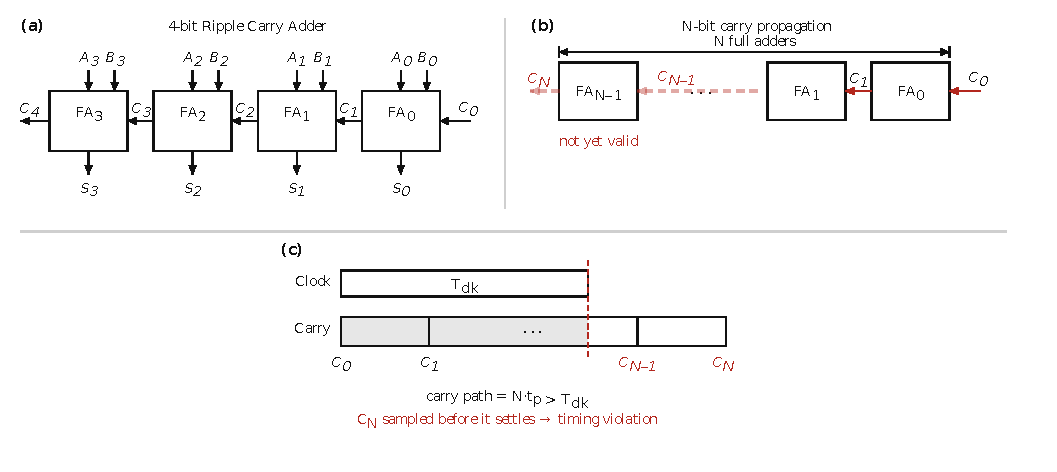
\includegraphics[width=1\columnwidth]{Figures/rca.pdf}
    \caption{\small Ripple Carry Adder used as the Circuit Under Test. In (a), a 4-bit RCA is shown as a cascade of full-adder stages, where the carry propagates from $C_0$ to $C_4$. In (b), the structure is generalized to an $N$-bit RCA, highlighting that the final carry $C_N$ remains invalid until the signal has propagated through all $N$ full adders. In (c), the corresponding timing behavior is shown: when the total carry-path delay $N \cdot t_p$ exceeds the clock period $T_{clk}$, $C_N$ is sampled before settling, resulting in a timing violation.}
    \label{fig:rca_cut}
\end{figure}

Figure~\ref{fig:rca_cut} illustrates the RCA structure and its carry-propagation timing behavior. Figure~\ref{fig:rca_cut}(a) shows a 4-bit RCA implementation, in which the full-adder stages $FA_0$ to $FA_3$ are cascaded in series. Each stage receives the corresponding operand bits $A_i$ and $B_i$, together with the carry generated by the previous stage, and produces a sum bit $S_i$ and a carry-out forwarded to the next stage. Figure~\ref{fig:rca_cut}(b) generalizes this structure to an $N$-bit configuration, where the carry signal propagates from $C_0$ to $C_N$ through $N$ full adders. Since each stage introduces a propagation delay $t_p$, the final carry $C_N$ remains invalid until the cumulative delay of the complete carry chain has elapsed. Figure~\ref{fig:rca_cut}(c) presents the corresponding timing diagram, showing the case in which the carry path delay, given by $N \cdot t_p$, exceeds the clock period $T_{clk}$. In this condition, $C_N$ has not yet settled at the active clock edge and is sampled prematurely, characterizing a timing violation.

The delay increase caused by aging reduces the effective slack available in this critical path. As this slack decreases, the RCA becomes progressively more susceptible to timing violations, meaning that the combinational result may fail to stabilize before being captured by the next rising clock edge. Under this condition, the output flip-flop can latch an incorrect value, producing a corrupted addition result. Therefore, the adopted CUT allows the sensor response to be related to a functional timing-failure scenario in the monitored datapath.

The 16-bit RCA is also a relevant experimental choice because its cascaded structure makes it sensitive to accumulated aging-induced delay degradation. Aging mechanisms such as Negative Bias Temperature Instability (NBTI) and Hot-Carrier Injection (HCI) act at the transistor level, gradually increasing device threshold voltage and degrading drive current. Although the delay contribution of each individual device is small, these contributions accumulate along the cascaded stages of the RCA critical path. Consequently, the RCA enables the observation of aging-induced timing erosion in a controlled arithmetic datapath.

Furthermore, the RCA represents a more realistic experimental target than a passive delay line, since it is an arithmetic structure with functional relevance in digital systems. Its 16-bit configuration provides a repeatable carry-propagation path with sustained switching activity, contributing to dynamic power dissipation and local self-heating effects during stress conditions. In this sense, the adopted CUT emulates relevant characteristics of arithmetic critical paths, while preserving a compact and controllable implementation for physical FPGA-based validation.


\subsection{On-Chip Experimental Architecture} \label{sec:onchip_experimental_architecture}

Figure~\ref{fig:diagram} presents the general architecture of the experimental platform implemented inside the FPGA. The architecture integrates the CUT, the proposed aging sensor, the clock management infrastructure, the Self-Calibration and Control Block (SCC Block), the XADC interface, and the communication interface used to transmit measurements to the host computer.

The Clock Manager is responsible for generating the clock signals used by the experimental platform. In particular, it provides the phase-shifted clock required by the aging sensor. The phase relationship between the monitored datapath clock and the sensor sampling clock is adjusted through the dynamic phase-shift capability of the MMCM. The SCC Block controls this adjustment by issuing phase-increment or phase-decrement commands to the Clock Manager.

The aging sensor is connected to the monitored path of the CUT. During operation, the CUT generates periodic transitions through the deterministic operand pattern described in Section~\ref{sec:circuit_under_test}. The sensor observes the timing behavior of this path and asserts an alarm when the monitored transition violates the configured sampling margin. This alarm is sent to the SCC Block, which interprets the event and updates the sensor calibration state.

The SCC Block is the central control unit of the on-chip platform. It receives the sensor alarm, manages the calibration procedure, stores the number of phase-shift increments required to position the sensor operating point, and provides this information to the host computer. The phase-shift count is used as the main digital indicator of the sensor response under voltage, temperature, and aging stress conditions.

The Xilinx XADC block is used to collect on-chip temperature and supply-voltage information during the experiments. These measurements are transmitted to the host computer together with the sensor phase-shift count and alarm information. This allows the experimental data to be correlated with the environmental and electrical operating conditions of the FPGA during each test.

A reset signal generated from the host side is also provided to the FPGA platform. This reset allows the experiment to be restarted between operating points, ensuring that each voltage or temperature condition begins from a known control state.

\begin{figure}[htbp!]
    \centering
    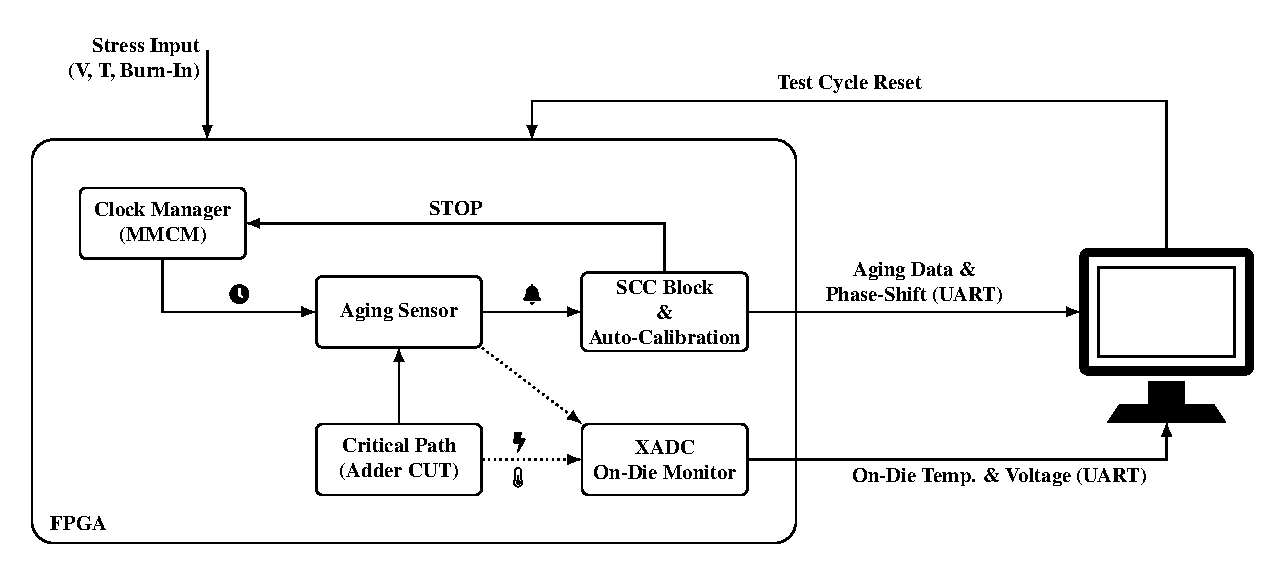
\includegraphics[width=1.0\columnwidth]{Figures/experiment_diagram.pdf}
    \caption{\small General architecture of the experimental setup implemented on the FPGA.}
    \label{fig:diagram}
\end{figure}


\subsection{Physical Experimental Setup} \label{sec:physical_experimental_setup}


To conduct the physical evaluation of the proposed sensor, the FPGA platform was exposed to controlled temperature variations, supply-voltage variations, and accelerated burn-in stress conditions. The physical test environment used in the experiments is shown in Figure~\ref{fig:setup}, which identifies the main instruments and hardware components involved in the measurement flow.

\begin{figure}[htbp!]
    \centering
    \includegraphics[width=1\columnwidth]{Figures/setup.pdf}
    \caption{\small Physical testing setup used for the aging sensor validation. The numbered labels identify the TLZ10 temperature controller (1), the IT6502D programmable power supply (2), the test host computer with real-time monitoring interfaces (3), the Nexys 4 DDR FPGA board (4), and the thermal aging oven EL 1.1 Odontobras used during accelerated stress experiments (5).}
    \label{fig:setup}
\end{figure}

The experimental setup comprises five main elements. The TLZ10 temperature controller, identified as element~(1), regulates the internal temperature of the thermal aging oven EL 1.1 Odontobras, identified as element~(5), which provides the controlled thermal environment required for temperature-sensitivity measurements and accelerated burn-in stress experiments. The IT6502D programmable power supply, shown as element~(2), externally adjusts the FPGA core voltage during voltage-sensitivity and burn-in experiments. The test host computer with real-time monitoring interfaces, identified as element~(3), configures the test procedure, resets the FPGA platform when required, and collects the experimental data. Finally, the Nexys 4 DDR FPGA board, shown as element~(4), contains the implemented CUT, the aging sensor, the SCC Block, the Clock Manager, and the XADC interface.

During each experiment, the host computer records the sensor response together with the operating conditions reported by the FPGA. The collected data include the number of phase-shift increments produced by the SCC Block, the sensor alarm behavior, the on-chip temperature, and the measured supply-voltage information provided by the XADC. This measurement flow enables the sensor response to be analyzed as a function of temperature, voltage, and accumulated aging stress.

The FPGA used for the experimental tests is an Artix-7 device implemented on the Nexys 4 DDR development board. The device is manufactured in a 28~nm CMOS technology and operates with a nominal core voltage of 1~V. The recommended operating ranges provided by the manufacturer were used as references to define the voltage and temperature conditions evaluated in this work~\cite{xilinxArtix7}. The on-chip temperature and voltage measurements were obtained using the Xilinx XADC infrastructure~\cite{xilinxUG480}, while the phase-shifted clock required by the proposed sensor was generated using the FPGA clock management resources~\cite{xilinxUG472}.

Figure~\ref{fig:fpga} illustrates the Nexys 4 DDR development board used as the physical testing platform, highlighting the main hardware elements involved in the experiments.

\begin{figure}[htbp!]
    \centering
    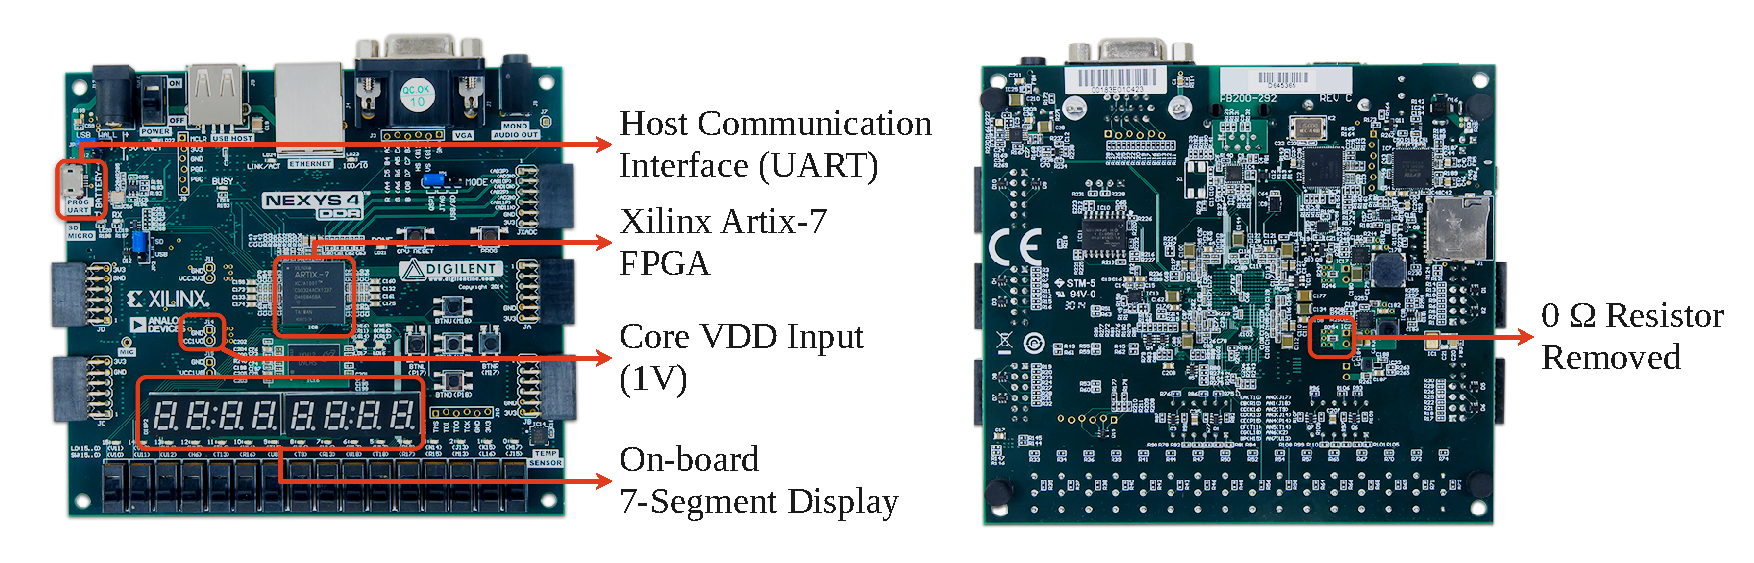
\includegraphics[width=1.0\columnwidth]{Figures/Placa_FPGA_Anotada.pdf}
    \caption{\small Nexys 4 DDR development board used as the physical testing platform.}
    \label{fig:fpga}
\end{figure}

As shown in Figure~\ref{fig:fpga}, the board houses the Xilinx Artix-7 FPGA, which implements the CUT, aging sensor, SCC Block, Clock Manager, and XADC interface. The host communication interface is established through a UART link, enabling configuration and data acquisition during the experiments. To allow precise control of the core supply voltage, the FPGA VDD rail (1\,V nominal) was isolated from the original board power network by removing a 0\,$\Omega$ resistor located on the back side of the PCB. This modification enabled direct voltage injection from the programmable power supply into the FPGA core domain during voltage-sensitivity and accelerated aging tests.


\section{Results and Discussion}\label{sec:results_and_discussion}



\subsection{Voltage and Temperature Sweep Tests}
\label{sec:voltage_temp_sweep}

As demonstrated by the semi-empirical model proposed in \cite{effects_on_time_response}, validated through electrical simulations in 65\,nm, 45\,nm, and 32\,nm CMOS technologies, supply voltage and temperature exert opposite effects on gate propagation delay. 


A reduction in \textit{VDD} leads to an increase in delay, whereas a rise in temperature results in a decrease in delay, primarily due to the non-linear behavior of carrier mobility.

Figure~\ref{fig:slack_por_temp}.A presents the results obtained by the sensor when maintaining a constant supply voltage while varying the FPGA core temperature. As expected, the increase in temperature results in an increase in critical path delay, indicating slower operation. Similarly, Figure~\ref{fig:slack_por_temp}.B shows the results obtained by maintaining a constant temperature while varying the core supply voltage. As anticipated, reducing the supply voltage leads to an increase in critical path delay.

\begin{figure}[htbp!]
    \centering
    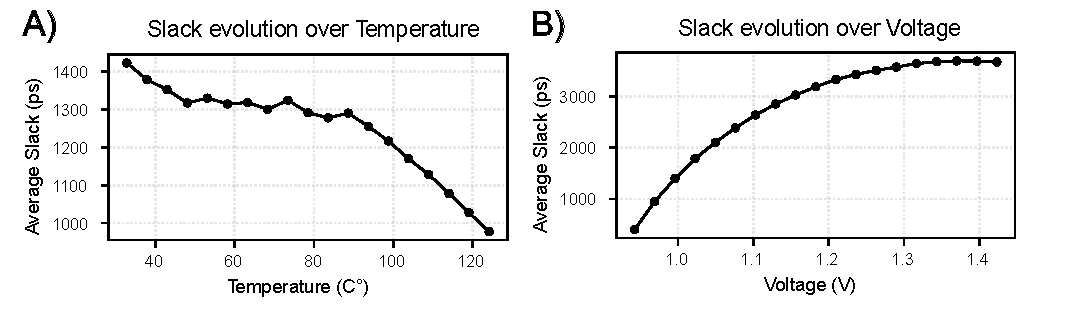
\includegraphics[width=1.0\columnwidth]{Figures/slack_graph.pdf}
    \caption{\small Critical path slack variation: (A) with temperature increase at constant supply voltage, and (B) with supply voltage reduction at constant temperature.}
    \label{fig:slack_por_temp}

\end{figure}




\subsection{Accelerated Aging through Burn-in Testing}
\label{sec:burnin_testing}

The accelerated aging procedure was conducted as follows. Initially, baseline measurements (Week 0) of the critical path performance, as observed by the aging sensor, were collected for each of the six defined operating corners.

Subsequently, the FPGA was subjected to a temperature of 115\,$^{\circ}$C and a +30\% increase in core supply voltage (\textit{VDD}) for one week. At the end of this first stress period (Week 1), the delay measurements for each corner were recorded again.

In order to induce a more significant level of aging, the stress conditions were intensified: the FPGA was exposed to a temperature of 125\,$^{\circ}$C and a +40\% \textit{VDD} increase for an additional week. At the end of this second burn-in period (Week 2), a final set of measurements was performed.

The slack evolution for each corner, along with the associated measurement conditions, is summarized in Table~\ref{tab:corner_delay_ps}. It is important to highlight that the aging conditions applied during the burn-in phases were different from the conditions under which each corner was measured.

The results obtained are consistent with theoretical expectations: corners combining low supply voltage and high temperature exhibited the lowest slack values (indicating slower paths), while corners with higher supply voltage and lower temperature presented the highest slack values (indicating faster paths).

%Additionally, although not the primary focus of this study, it was observed that corners operating at higher voltages exhibited smaller slack variations over time, suggesting a lower aging rate.

\begin{table}[htb!]
    \centering
    \footnotesize
    \caption{Slack in picoseconds (ps) for each corner, measured at Week 0, Week 1, and Week 2.}
    \label{tab:corner_delay_ps}
    \begin{tabular}{lccccc}
        \toprule
         \textbf{Corner} & \textbf{\shortstack{Temp.\\(°C)}} & \textbf{\shortstack{Voltage \\(V)}} & \textbf{\shortstack{Week 0 \\(ps)}} & \textbf{\shortstack{Week 1 \\(ps)}} & \textbf{\shortstack{Week 2\\ (ps)}} \\
        \midrule
        Corner1 & 85 & 0.950 & 744   & 613 & 357\\
        Corner2 & 85 & 1.000 & 1518  & 1355 & 1113\\
        Corner3 & 85 & 1.050 & 1975  & 1897 & 1681\\
        Corner4 & 33 & 0.950 & 704   & 649 & 234\\
        Corner5 & 33 & 1.000 & 1607  & 1488 & 1208\\
        Corner6 & 33 & 1.050 & 2233  & 2139 & 1887\\
        \bottomrule
    \end{tabular}
    
\end{table}


\subsection{Continuous In-Situ Monitoring Under Sustained Stress}
\label{sec:continuous_monitoring}

To complement the discrete corner measurements reported in Table~\ref{tab:corner_delay_ps}, the aging sensor was also operated continuously, without any manual intervention, throughout a sustained accelerated-stress exposure. In this test, the FPGA core was continuously supplied with an overvoltage close to the \mbox{+40\%} \textit{VDD} condition used during the Week~2 burn-in period (on-chip supply voltage of 1.400\,$\pm$\,0.001\,V, measured through the XADC), while the thermal chamber air temperature was regulated to 93.9\,$\pm$\,1.8\,$^{\circ}$C. The resulting self-heating raised the FPGA junction temperature, as reported by the on-chip sensor, to 125.1\,$\pm$\,1.8\,$^{\circ}$C (range 117--134\,$^{\circ}$C), matching the target device temperature adopted for the most aggressive burn-in corner. Under these conditions, the sensor logged its self-calibrated slack value once per second for approximately 212.6 continuous hours (8.9 days).

Figure~\ref{fig:continuous_monitoring} presents the recorded oven temperature, core supply voltage, and sensor slack over the full test duration. After an initial transient of about two hours, corresponding to the thermal ramp-up of the chamber, all three quantities settle into a stable operating band: the oven temperature oscillates within its PID control band (89.5--103.6\,$^{\circ}$C), the supply voltage remains within 100\,mV of its stressed operating point, and the sensor slack fluctuates within a narrow 33\,ps peak-to-peak band around a mean of 278.5\,$\pm$\,3.0\,ps. Because the sensor recalibrates autonomously through the dynamic phase-shift mechanism described in Section~\ref{sec:sensor_autotuning}, this stable tracking was sustained without any manual re-tuning of the sampling clock over the nearly nine-day test, directly supporting the mission-mode self-calibration behavior identified as contribution C2 in this work. The residual slack variability observed in this window is consistent with the combined effect of thermal and supply-voltage ripple on path delay, rather than with additional aging, since the corner-sweep results of Section~\ref{sec:voltage_temp_sweep} already show that comparable temperature and voltage fluctuations produce slack variations of similar magnitude.

\begin{figure}[htbp!]
    \centering
    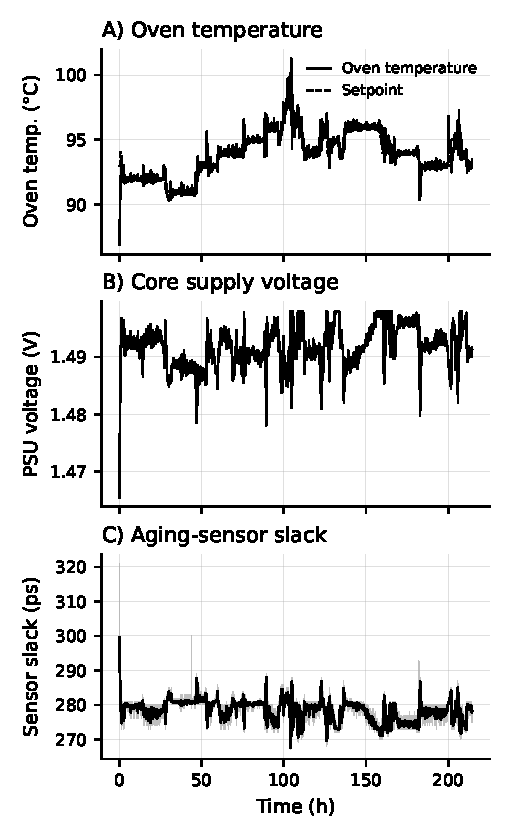
\includegraphics[width=1.0\columnwidth]{Figures/continuous_monitoring.pdf}
    \caption{\small Continuous in-situ monitoring over a sustained $\approx$212.6-hour stress exposure: (A) oven air temperature and PID setpoint, (B) FPGA core supply voltage, and (C) aging-sensor slack (mean in black; sample min--max envelope shaded in gray). The sensor tracked slack autonomously throughout, without manual recalibration.}
    \label{fig:continuous_monitoring}
\end{figure}


\subsection{Functional Failure Point Characterization}

Critical path failure occurs when a timing violation occurs, that is, when the calculation time of a combinational circuit exceeds the clock period. This is crucial for our sensor, as detecting a timing violation only after the sensor indicates a 0ps slack time serves as an effective validation method.


 Figure~\ref{fig:failure_point} illustrates the signal states at the start and the end of the critical path, just before the final flip-flop. A D flip-flop, acting as the \textit{failure catcher}, is employed for detecting the failure point. This element captures the XOR result between the Q outputs at the start and end of the critical path. The \textit{failure catcher} triggers on the positive edge of the Q output at the critical path’s end. If the end goes HIGH, the \textit{failure catcher} will only register HIGH if the starting flip-flop is LOW, due to the XOR gate.

 \begin{figure}[htbp!]
     \centering
     
\includegraphics[width= 1.0 \columnwidth]{Figures/failure_point_.pdf}
     \caption{\small Illustration of the signal behavior at the start and end of the critical path. A mismatch detected by the failure catcher indicates a timing violation due to insufficient slack.}

     \label{fig:failure_point}
 \end{figure}

As demonstrated, the signals differ only in the event of a timing violation, where the signal has not fully propagated by the time the positive clock edge occurs. 

This setup was validated experimentally by inducing a timing failure via voltage reduction, and the failure point was correctly detected by our sensor, with a small margin of error due to clock jitter and flip-flop routing skew.

\section{Conclusions and Future Work} \label{sec:conclusion}


The performance and behavior of the proposed sensor were consistent with expectations based on the validation tests and procedures discussed in this work. These results provide strong support for the use of the sensor as an important tool for Silicon Lifecycle Management (SLM) applications.

Within this context, the information regarding the evolution of circuit aging could be leveraged by applying predictive techniques similar to those employed by \cite{chen2022solar_prediction}, but adapted to forecast the aging rate and estimate the time to failure based on the sensor's data.

Furthermore, these results open the possibility for future integration of predictive models aimed at degradation mitigation and lifetime forecasting, following strategies explored in works such as \cite{CNNfabian}, where on-chip sensors (e.g., temperature, soft-error rate, and aging monitors) are used to guide system reconfiguration and activity management to reduce aging effects. Compared to such approaches, our proposed sensor provides more accurate slack information and enables direct estimation of the aging rate, offering enhanced capabilities for predictive maintenance.


 
%\section*{Acknowledgment}

%The preferred spelling of the word ``acknowledgment'' in America is without 
%an ``e'' after the ``g''. Avoid the stilted expression ``one of us (R. B. 
%G.) thanks $\ldots$''. Instead, try ``R. B. G. thanks$\ldots$''. Put sponsor 
%acknowledgments in the unnumbered footnote on the first page.




\bibliographystyle{IEEEtran}
\bibliography{bibfile}


\end{document}
